\documentclass[12pt, twoside]{report}

\usepackage{multicol}
\usepackage{amsmath}

%% comment this line for handouts. Uncomment for lecture notes
%\newcommand{\lectureNoteMode}{}

\raggedbottom

\usepackage{color, xifthen, amsthm, amssymb, amsmath, tikz, pgfplots}
\pgfplotsset{compat=1.18}
\usetikzlibrary{backgrounds}
\usepackage[letterpaper, margin=1in]{geometry}
\usepackage{multicol}
\usepackage{fourier}  %don't use txfonts b/c the sf doesn't look good

\usepackage{enumitem}
\setlist{topsep=-\parskip/2}


\setlength{\parindent}{0pt}
\setlength{\parskip}{\baselineskip}


\usepackage{mdframed} % makes better frames around examples (eg pagebreak allowed)
  % from mdframed package. used for examples
\newmdenv[
  skipabove=10pt,%\topsep,
  skipbelow=10pt,%\topsep
  ]{allrules}

\usepackage{tcolorbox} % for colored boxes


\usepackage{subfigure}
\usepackage{hyperref}
\hypersetup{colorlinks, urlcolor=red, linkcolor=.} %color urls, but not interal refs
\usepackage{graphicx, floatflt}
\graphicspath{{./figs/}{../figs/}}
\DeclareGraphicsExtensions{.png,.jpg,.pdf}

\usepackage{wrapfig}  %useful for wrapping text around pictures or tables
		      %though it doesn't do a great job inside my example boxes


\definecolor{defbod}{rgb}{.8,.8,.8}     \definecolor{defhead}{rgb}{.7,.1,.1}
\definecolor{thmbod}{rgb}{.8,.8,.8}     \definecolor{thmhead}{rgb}{.1,.1,.9}
\definecolor{factbod}{rgb}{1,1,1}    \definecolor{facthead}{rgb}{.1,.7,.1}
\definecolor{exbod}{rgb}{1,1,1}         \definecolor{exhead}{rgb}{0,.3,0}
\definecolor{soltext}{rgb}{.2,.2,.5}
\definecolor{notebod}{rgb}{.9,.9,.9}    \definecolor{notehead}{rgb}{.1,.1,.7}

\newcommand{\defn}[1]{
 \noindent \colorbox{defbod}{\begin{minipage}{.95\linewidth}
 \hspace{-12pt}\colorbox{defhead}{\sf\color{white} Definition}
 #1
 \end{minipage} } \medskip
 }
\newcommand{\dt}[1]{\textcolor{defhead}{\bfseries #1}}

\newcommand{\thrm}[1]{
 \noindent \colorbox{thmbod}{\begin{minipage}{.95\linewidth}
 \hspace{-12pt}\colorbox{thmhead}{\sf\color{white}Theorem}
 #1
 \end{minipage} } \medskip
 }
\newcommand{\coro}[1]{
 \noindent \colorbox{thmbod}{\begin{minipage}{.95\linewidth}
 \hspace{-12pt}\colorbox{thmhead}{\sf\color{white}Corollary}
 #1
 \end{minipage} } \medskip
 }
\newcommand{\fact}[1]{  %%%% !! note this different from calcnotes
 \noindent \begin{allrules}
 #1
 \end{allrules} \medskip
 }

\newcommand{\note}[1]{
	\noindent \colorbox{notebod}{\begin{minipage}{.95\textwidth}
			\hspace{-12pt}\colorbox{notehead}{\sf\color{white}NOTE}
			#1
	\end{minipage} } \medskip
}


% making the example thing with a line down the left.
\newmdenv[
rightline=false,
bottomline=false,
skipabove=0pt,%\topsep,
skipbelow=0pt,%\topsep
]{siderules}

\newcommand{\ex}[1]{
  \noindent \begin{siderules}
    \textcolor{exhead}{\sf Example}
    #1
  \end{siderules} 
  \medskip
}




%%%%%%%%%% set it up so that these are not displayed when 
%%%%%%%%%% printing notes for students?  or for overhead?
\newcommand{\exsol}[1]{
  {\color{soltext} #1}
}

\newcommand{\mynonumsect}[2][]{
 \cleardoublepage
 \section*{#1\hskip16pt #2}
 \addcontentsline{toc}{section}{#1 #2}
}

\newcommand{\myhead}[1]{
\par%\vskip\baselineskip
\noindent
{\large\bf #1}
}

%%%%%%%%%%%%%%%%%%%%%%%%
% symbol shortcuts

\newcommand{\nice}{\displaystyle}
\newcommand{\eqq}{\ensuremath \stackrel{?}{=}}
\newcommand{\R}{\ensuremath{\mathbb{R}}}




% %%%%%%%%%%%%%%%%%%%%%%%%
% %
% % Creating handouts vs notes
% %% If you use the line below before loading this file then it will be set up for
% %% lecture notes.  Default is for handouts
% %%
% %% \newcommand{\lectureNoteMode}{}
% %%
% %% do not uncomment here, just add the line to the file where you input this one.
% \ifthenelse{\not\isundefined\lectureNoteMode}
% { % lecture notes 
%   \newcommand{\Hvskip}[1]{}
%   \newcommand{\Hvfill}{}
%   \newcommand{\Hpbreak}{}  % pagebreaks for handouts
%   \newcommand{\Npbreak}{\vfill\pagebreak} % pagebreaks for printable notes
%   \newcommand{\Nonly}[1]{#1} % shows in notes, not in handouts
%   \newcommand{\mycleardoublepage}{\cleardoublepage}

%   \newcommand{\ex}[1]{
%    \noindent \begin{allrules}
%     \textcolor{exhead}{\sf Example}\par
%     #1
%     \end{allrules} \medskip
%   }

% } 
% { 
% %% Handout mode 
% %% this section sets it up with smaller margins, and blank spots for writing solns to examples
%   %%%%%%%%%%%%%%%%%%%%%%%%%%%%%%%%%%%%%%%%%%
%   %change frame around examples
%   % from mdframed package
%   \newmdenv[
%   rightline=false,
%   bottomline=false,
%   skipabove=0pt,%\topsep,
%   skipbelow=0pt,%\topsep
%   ]{siderules}
  
%   \newcommand{\ex}[1]{
%     \noindent \begin{siderules}
%       \textcolor{exhead}{\sf Example}
%       #1
%     \end{siderules} 
%     \medskip
%   }
  
%   %
%   %%%%%%%%%%%%%%%%%%%%%%%%%%%%%%%%%%%%%%%%%%
  
%   % don't show solutions for examples
%   \renewcommand{\exsol}[1]{}
  
%   %used for making blank space in handouts. eg: \vs2
%   \newcommand{\Hvskip}[1]{\vskip#1in\null}
%   \newcommand{\Hvfill}{\vfill} %vfill only in handouts mode
%   \newcommand{\Hpbreak}{\pagebreak} % pagebreaks for handouts
%   \newcommand{\Npbreak}{} % pagebreaks for printable notes
%   \newcommand{\Nonly}[1]{} % shows in printable, not in handouts
%   \newcommand{\mycleardoublepage}{\newpage} % don't need blank pages if not printing
  
%   % don't really need margins since not printing.
%   \geometry{margin=0.75in}

%   \renewcommand{\mynonumsect}[2][]{
%     \mycleardoublepage
%     \section*{#1\hskip16pt Handout: #2}
%     \addcontentsline{toc}{section}{#1 #2}
%   }

% } 





\setlength{\parindent}{0pt}

\setcounter{chapter}{1}
\begin{document}


\mynonumsect[1.4]{Linear Functions}

\textbf{Goal:} To determine formulas for linear functions and describe their behaviors using slope


Let's use the example from our book (p27) to understand linear functions:

\ex{As you hop into a taxicab in Las Vegas, the meter will immediately read $\$3.30$; this is the “drop” charge made when the taximeter is activated.  After that initial fee, the taximeter will add $\$2.60$ for each mile the taxi drives .  In this scenario, the total taxi fare depends upon the number of miles ridden in the taxi, and we can ask whether it is possible to model this type of scenario with a function. 

Using descriptive variables, we choose $m$ for miles and $C$ for Cost in dollars as a function of miles: $C(m)$. Determine: \\
\begin{itemize}
	\item $C(0)=$ \hrulefill \\
	\item $C(1)=$ \hrulefill \\
	\item $C(2)=$ \hrulefill \\
	\item $C(3)=$ \hrulefill \\
	\item $C(m)=$ \hrulefill \\
\end{itemize}


Notice this equation consists of two quantities: \\
\begin{enumerate}
	\item \dt{Fixed value}: \hrulefill \\
	\item \dt{Rate of Change}: \hrulefill \\ \\
	**************************************** IMPORTANT NOTE **************************************** \\ \\
	It is important here to note that in this equation, the \underline{Rate of Change is \hskip1.75in}. \\ \\
	That is, over any interval, the rate of change is the \underline{\hskip1.5in}. \\ \\
	******************************************************************************************************* 
\end{enumerate}
}




\pagebreak


\begin{multicols}{2}
	Graphing this equation, we see the shape is a line, which is how these functions get their name: \\ \dt{linear functions}
	
	When the number of miles is zero the cost is $\$3.30$, giving the point $(0, 3.30)$ on the graph.  This is the \dt{vertical or $y$-intercept}.  
	
	The graph is increasing in a straight line from left to right because for each mile the cost goes up by $\$2.40$; this rate remains consistent.
	
	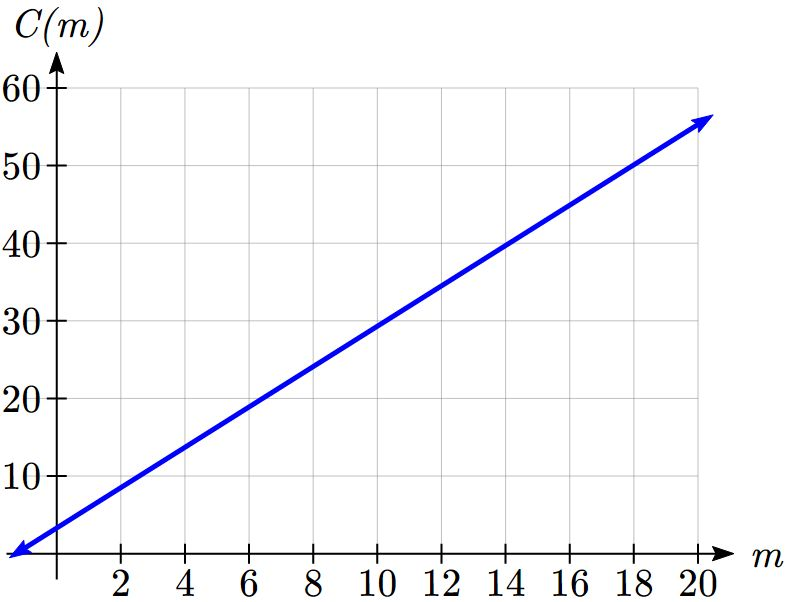
\includegraphics[alt={Line graph of taxi fare versus miles ridden, showing a y-intercept above zero and a constant positive slope.}, width=3in]{105_1.4_figure1.jpg}
\end{multicols}


\defn{A \dt{Linear function} is a function whose graph produces a line.  Linear functions can always be written in the form:
	
\begin{center}
	$f(x) = b+mx$ \hskip0.5in or \hskip0.5in $f(x) = mx +b$ \vskip12pt
	(They are equivalent!)
\end{center}

where:
\begin{itemize}
	\item $b$ is the initial or starting value of the function (when input, x = 0)
	\item $m$ is the constant rate of change of the function, called \dt{slope}
\end{itemize} 
}
\vskip12pt

\fact{
The slope determines the behavior of the function: \\

\begin{tabular}{|c|p{2in}|p{4in}|}
	\hline 
	Slope & Behavior & Graph \\
	\hline 
	&&\\
	&&\\
	$m>0$ & & \\
	& & \\
	&&\\
	\hline 
	&&\\
	&&\\
	$m<0$ & & \\
	& & \\
	&&\\
	\hline
	&&\\
	&&\\
	$m=0$ & & \\
	& & \\
	&&\\
	\hline
	
\end{tabular}
}

\pagebreak

Write the equation of the line in slope-intercept form with the given characteristics:

\begin{enumerate}
	\item
	Slope is 8 and $y$-intercept is $(0,3)$. \vfill

	\item
	Slope is $- 5$ and $y$-intercept is
	$(0, - 6)$. \vfill
	
	\item
	Slope is $\frac{3}{7}$ and passes through the point $( - 14,2)$. 
	\vfill \vfill 

	\item
	Slope is $\frac{- 4}{5}$ and passes through the point $(2, - 3)$. 
	\vfill \vfill 
\end{enumerate}



\ex{To start producing a new model of custom wheels, a company will have to purchase $\$30,000$ in new equipment.  Each wheel made costs them $\$40$ in supplies and labor.  \\
Write a formula for the total cost, $TC$, of producing $q$ wheels. \\
What will be their total costs in the first year if they expect to sell 240 wheels?
}
\vfill \vfill 





\pagebreak


\defn{\dt{Calculating the Rate of Change (or Slope):}

Given two values for the input, $x_1$ and $x_2$, and two corresponding values for the output, $y_1$ adn $y_2$,  or a set of points, $(x_1,y_1)$ and $(x_2, y_2)$, if we wish to find a linear function that contains both points we can calculate the rate of change, or slope $m$:

\begin{center}
	$m= \dfrac{\text{change in output}}{\text{change in input}} = \dfrac{\hskip0.75in}{\hskip0.75in} = \dfrac{\hskip1.5in}{\hskip1.5in}$
\end{center}
\vskip12pt
}


Write the equation of the line in slope-intercept form with the given characteristics:

\begin{enumerate}
\item
Passes through the points $({0, -6})$ and $(1,0)$. \vfill

\item
Passes through the points $(-1,5)$ and $(2, 5)$. \vfill

\item
Passes through the points $(4,8)$ and $(4,7)$. \vfill




\end{enumerate}


\ex{The population of a city increased from 23,400 to 27,800 between 2002 and 2006. \\
Find the rate of change of the population during this time span.
}
\vfill \vfill 

\pagebreak


\ex{Let $f(x)$ be a linear function with $f(5)=-3$ and $f(2)=7$. \\
	\begin{enumerate}
		\item Write the two given values as coordinates: \hrulefill 
		
		\item Find the Slope or Rate of Change. \hrulefill 
		
		\item Is this function increasing or decreasing? Why?\hrulefill 
		
		\item Write an equation for the function. \hrulefill 
	\end{enumerate}
}

\vfill

\ex{Working as an insurance salesperson, Ilya earns a base salary and a commission on each new policy, so Ilya’s weekly income, $I$, depends on the number of new policies, $n$, he sells during the week.  Last week he sold 3 new policies, and earned $\$760$ for the week.  The week before, he sold 5 new policies, and earned $\$920$.  \\
Find an equation for $I(n)$, and interpret the meaning of the components of the equation.
}
\vfill 


\pagebreak

\myhead{Additonal Practice}

\begin{enumerate}
	
	\item We are given the two points $(2, 3)$ and $(0, 4)$.
	\begin{enumerate}
		\item Find the rate of change (slope).  
		\item Is this function increasing or decreasing? Explain.
	\end{enumerate} 
	\vfill 
	
	\item Let $f(x)$ be a linear function with $f(3)=-2$, and $f(8)=1$.
	\begin{enumerate}
		\item Find the rate of change.
		\item Find an equation for the function.
	\end{enumerate}
	\vfill



\pagebreak

	\item The pressure, $P$, in pounds per square inch (PSI) on a diver depends upon their depth below the water surface, $d$, in feet, following the equation $P(d)=14.696+0.434d$. \\
	Interpret the components of this function.
	\vfill
	
	\item The balance in your college payment account, $C$, is a function of the number of quarters, $q$, you attend.  
	\begin{enumerate}
		\item Interpret the function $C(a) = 20000 – 4000q$ in words.  
		\item How many quarters of college can you pay for until this account is empty?
	\end{enumerate}
	\vfill 

	

\end{enumerate}


\end{document}
